\subsection{Composition d'un \textbf{A}utomate \textbf{P}rogrammable \textbf{I}ndustriel (\textbf{API})}
Un {\textbf{A}utomate \textbf{P}rogrammable \textbf{I}ndustriel (\textbf{API})} est un système informatique industriel adapté aux besoins de l'industrie. Sa structure est donc similaire à celle d'un ordinateur personnel (PC) en cela qu'il est composé d'un processeur et de mémoires dédiées à des usages que nous allons développer. 

\begin{UPSTIactivite}[][Structure d'un API]
    Représenter sous forme schématique un automate industriel
    \begin{center}
        \UPSTIprofEleve{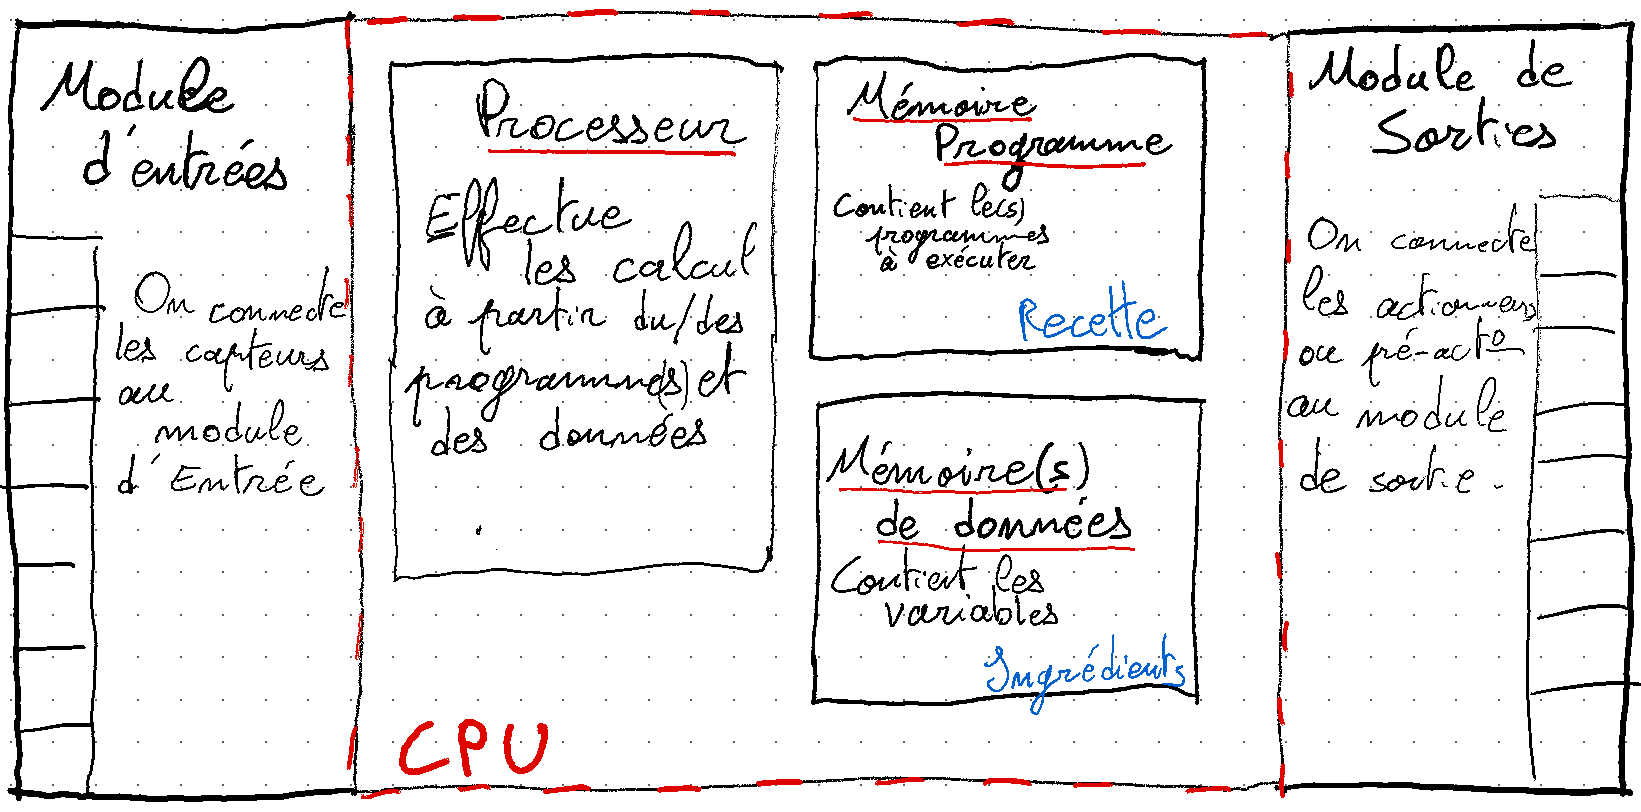
\includegraphics[height=.34\textheight]{images/API}\vspace{.06\textheight}}{\vspace{0.4\textheight}}
    \end{center}   

\end{UPSTIactivite}

Les modules d'entrées-sorties viennent se relier à la CPU en vue de faire le lien avec les capteurs et les actionneurs du système. On qualifie ces automates de \textbf{modulaire} et il est possible d'ajouter un nombre important de module (TOR, analogique, pour sonde de température, etc.) afin d'adapter l'automate aux besoins spécifiques de l'industrie. Un exemple d'automate modulaire \textit{Schneider} est donné en Figure~\ref{fig:schneider}. 

Pour des applications simples, certains constructeurs ont développé des automates \textbf{Monobloc} contenant directement des entrées-sorties sur le bloc de CPU. C'est le cas du LOGO de chez \textit{Siemens} que nous utiliserons en TP (Figure~\ref{fig:logo}). Sur ces automates, il est souvent possible d'ajouter des extensions afin de multiplier le nombre d'entrées et de sorties. 

\begin{figure}[ht]
    \centering
    \begin{subfigure}{0.49\textwidth}
        \centering
            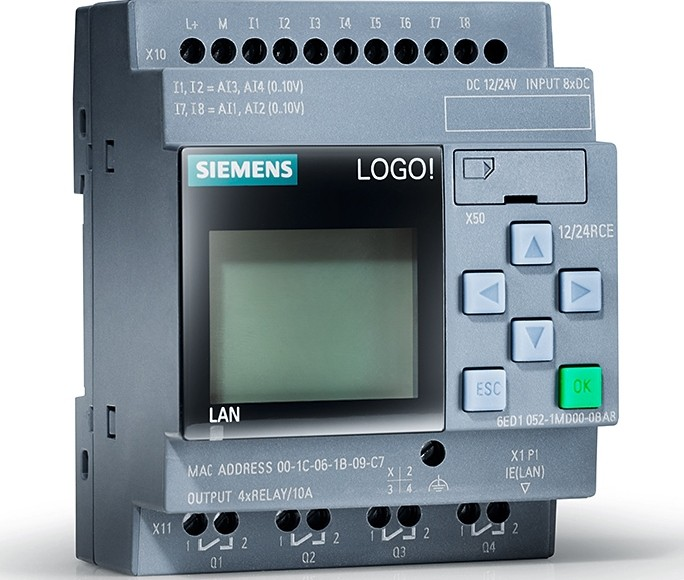
\includegraphics[width=.6\textwidth]{images/logo-v8-siemens}
            \caption{Automate Monobloc : Siemens LOGO}
            \label{fig:logo}
    \end{subfigure}%
    \begin{subfigure}{0.49\textwidth}
        \centering
            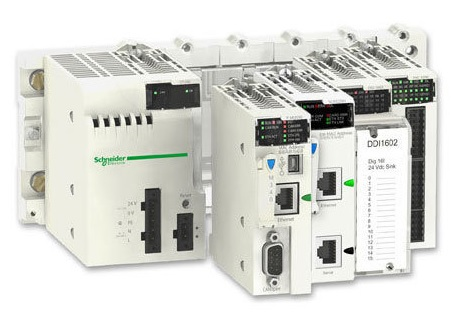
\includegraphics[width=.8\textwidth]{images/api-schneider}
            \caption{Automate Modulaires : Schneider}
            \label{fig:schneider}
    \end{subfigure}%
    \caption{Exemples d'automates monoblocs et modulaires}
\end{figure}

\UPSTIaRetenir{%
Les \textbf{\color{red} capteurs} du système sont reliées aux \textbf{\color{red} modules d'entrées} de l'API.\\
Les \textbf{\color{green} actionneurs} et les \textbf{\color{green} pré-actionneurs}  du système sont reliées aux \textbf{\color{green} modules de sortie} de l'aPI.\\
Les automates \textbf{monoblocs} contiennent des modules d'entrées-sorties incorporé au bloc CPU. À l'inverse, sur un automate \textbf{modulaire} il est nécessaire d'ajouter les modules en fonction des besoins de l'application.}

